\documentclass[a4paper]{article}

\usepackage{color}
\usepackage{url}
\usepackage[T2A]{fontenc} 
\usepackage[utf8]{inputenc} 
\usepackage{graphicx}



\usepackage[english,serbian]{babel}


\usepackage[unicode]{hyperref}
\hypersetup{colorlinks,citecolor=green,filecolor=green,linkcolor=blue,urlcolor=blue}


\newtheorem{primer}{Primer}[section]



\begin{document}

\title{David Bader\\ \small{Seminarski rad u okviru kursa\\Tehničko i naučno pisanje\\ Matematički fakultet}}

\author{Nikola Belaković \\ nidzoteri@gmail.com \and
 Vojkan Panić \\ vojkan.panic@gmail.com \and
 Filip Antonijević \\ filipdantonijevic@gmail.com \and
 Bogdan Damljanović \\  bdamljanovic0@gmail.com } 	
\date{05.~novembar 2019.}


\maketitle



\abstract{\textbf{David A. Bader} (rođen 4. maja 1969.) ugledni je profesor i direktor Instituta za nauku o podacima na Tehnološkom institutu u Nju Džersiju \cite{njit}. Ranije je bio profesor, predsedavajući Škole računarske nauke i inženjerstva i izvršni direktor računarstva visokih performansi na računarskom fakultetu u Džordžiji \cite{cell}.  Pored toga, Bader je izabran za direktora prvog Soni Tošibinog centra za kompetenciju za mikroprocesor na Računarskom fakultetu na Tehnološkom institutu u Džordžiji. On je saradnik IEEE-a \cite{ieee} \cite{ece} \cite{awards}, AAAS-ov saradnik \cite{aaas}, SIAM-ov saradnik \cite{siam}. Bader je vodeći stručnjak za nauke o podacima. Njegova glavna područja istraživanja nalaze se na preseku računarstava visokih performansi i aplikacija koje pomažu u svakodnevnom životu, uključujući bezbednost na internetu, masovnu analitiku i računsku genomiku.

Bader je stručnjak za dizajn i analizu paralelnih i višejezgarnih algoritama za aplikacije u stvarnom svetu, poput onih u bezbednosti na internetu i računskoj biologiji. Dobitnik je nagrade od IBM-a \cite{ibm}, Majkrosoftovih istraživanja \cite{micaw}, Envidia  \cite{gtuc} \cite{nvid}, Fejsbuk \cite{fb}, Intel \cite{int} i Soni. Ko-predsedavao je nizom sastanaka \cite{ben}. Bio je prepoznat kao jedan od najuticajnijih autora u istoriji međunarodne konferencije IEEE o računarima visokih performansi, podacima i analitikama (HiPC) u 2018 \cite{hipc}.


\tableofcontents

\newpage


\section{Rani život}
Bader je sin profesora hemije Morisa Badera i njegove supruge Karen \cite{kar}. On je izviđač orao u Mladim izviđačima iz Amerike, koji je ovo ime dobio 1985. Bader je diplomirao na Liberty High School u Betlehemu u Pensilvaniji 1987. Postao je diplomirani inženjer iz oblasti računarskog inženjerstva 1990. i magistrirao na elektrotehnici 1991. sa Univerziteta Lihaj u Betlehemu, Pensilvanija  \citep{pen}. Potom je doktorirao elektrotehničko inženjerstvo 1996. na Univerzitetu u Merilendu, Studentski Park. Dok je bio na UMD-u 1992. godine, Bader je dobio NASA-inu stipendiju Gerald Sofen-a, naučnika projekta vikinških misija na Mars, u Centru za svemirske letove Godard \cite{nasa}.

\section{Karijera}
Od 1998. do 2005. Bader je bio profesor i regentski predavač na Univerzitetu u Novom Meksiku. 2005. godine prešao je u Georgia Tech, gde je bio profesor i obavljao funkciju prvog predsedavajućeg Škole računarske nauke i inženjerstva (CSE) od jula 2014. do juna 2019. U julu 2019. godine Bader se pridružio Tehnološkom institutu u Nju Džersiju kao ugledni profesor na katedri za računarske nauke Fakulteta računarstva Ying Wu. Služio je u brojnim programskim odborima konferencije koji se odnose na paralelnu obradu, uređivao je brojne časopise, objavio je brojne članke i bio je član IEEE-a, član AAAS-a, član SIAM-a i član ACM-a.

U oktobru 2018. godine Bader je imenovan za glavnog urednika transakcija ACM-a za paralelno računanje. Bio je glavni urednik transakcija IEEE za paralelne i distribuirane sisteme (TPDS), od 2013-2017. i bio je pomoćnik glavnog urednika časopisa za paralelno i distribuirano računanje (JPDC). Bader je bio pridruženi urednik IEEE transakcija na paralelnim i distribuiranim sistemima, IEEE DSOnline, paralelnom računarstvu i ACM Journal of Experimental Algorithmics, a objavio je preko 210 članaka u časopisima i konferencijama sa recenzijom.

Bader je bio vodeći istraživač na projektu Nvidia Echelon, primio je nagradu DARPA u iznosu od 25 miliona dolara, putem programa sveprisutnog računanja visokih performansi (UHPC). Četvorogodišnja istraživačka saradnja sa Envidijom obuhvatila je rad na razvoju novih GPU tehnologija potrebnih za izgradnju nove klase vrhunskih superkompjutera.

U novembru 2006. Badera su odabrali Soni, Tošiba i IBM da režira prvi Centar kompetencija za mikroprocesor. Bader je izabran za člana IEEE-a 2009. godine. Od 2011. godine sarađuje sa Džordžijskim institutom za tehnološka istraživanja na proaktivnom otkrivanju insajderskih pretnji koristeći grafičku analizu i učenje.

29. jula 2015. godine, predsednik Barak Obama najavio je Nacionalnu inicijativu za strateško računanje (NSCI). Bader je pozvan od strane Bele kuće od 20. do 21. oktobra 2015. godine u svojstvu panelista na radionici Nacionalne inicijative za strateško računarstvo Bele kuće (NSCI). Nakon toga, Kancelarija za nauku i tehnološku politiku Bele kuće (OSTP) pozvala je Badera da radi kao panelista u Internacionalnoj radnoj grupi za računarstvo visokog nivoa (NECRD) (IVG) i Starije upravljačke grupe za velike podatke (SSG) „Superkompjuterstvo i velika količina podataka: Od sudara do konvergencije" Panel, na 27. IEEE i ACM konferenciji o super računarstvu (SC15), Austin, TKS, 18. novembra 2015. 29. jula 2016., Bader je bio pozvani učesnik Nacionalne inicijative za strateško računanje Bele kuće ( NSCI) Jubilarna radionica.

Bader je suosnivao list Graph500 za vrednovanje računarskih platformi "Big Data".

U aprilu 2019. godine najavljeno je da će Bader i njegov laboratorij u Georgia Tech-u partneriti sa Envidiom da razviju rešenja za analizu podataka za svoje GPU-e.

U julu 2019. Tehnološki institut u Nju Džersiju objavio je da će Bader obavljati funkciju direktora svog novoosnovanog Instituta za nauku o podacima na računarskom fakultetu Ying Wu. Institut za nauku o podacima objedinjuje postojeće istraživačke centre za velike podatke, medicinsku informatiku i sigurnost na internetu pri NjIT-u, sprovodeći i osnovna i primenjena istraživanja.

\section{Nagrade}
U junu 2010. godine Intel je podržao Bader-ovo istraživanje o analitikama grafova trogodišnjom nagradom ureda za istraživački rad kompanije Intel Labs Academic Research Office for the Parallel Algorithms for Non-Numeric Computing Program.

Bader je dobitnik nagrade NSF CAREER. 2011. godine imenovan je članom AAAS-a i IEEE-a. InsideHPC ga je 2011. godine takođe proglasio za „Rock Star of High Performance Computing“, a za člana "People to Watch" proglašen je od strane HPC Wire-a u 2012. i 2014.Imenovan je za člana SIAM-a 2019. godine.

Odeljenje za elektrotehniku i računarsko inženjerstvo na Univerzitetu Mariland predstavilo je Badera kao prvog dobitnika njihove istaknute nagrade Alumni u 2012. godini. U 2019. godini Bader je dobio nagradu Facebook AI System Hardware/Software Co-Design Research Award to develop "high-performance AI solutions for existing as well as future AI hardware."

Na Georgia Tech-u, Bader je primio nekoliko priznanja i nagrada, uključujući Dekanovu nagradu 2007. i izvanrednu nagradu za istraživanje seniorskog fakulteta u 2014. godini.

Bader je Golden Core član IEEE Computer Society (2010), i dobitnik je nagrade IEEE Computer Society Meritorious Service (2010).

\section{Privatni život}
Bader ima jednu kćer, Sadi Rouz, koja je strastvena umetnica.

\newpage

\section{Slika i tabela}
\begin{table}[h!]
\begin{center}
\begin{tabular}{|l|l|} \hline
\multicolumn{2}{|c|}{\raisebox{0.6em} {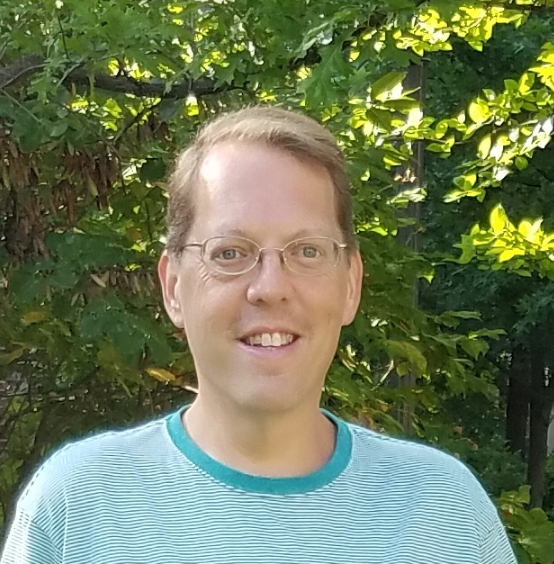
\includegraphics[scale=0.45]{David_Bader_2017.png}}}\\
\multicolumn{2}{|c|}{David Bader}\\ \hline
\textbf{Datum rođenja} & 4. maj 1969.\\ \hline
\textbf{Mesto rođenja} &	Betlehem, PA, SAD\\ \hline
\textbf{Polje} & Računarstvo visokih performansi\\ \hline
\textbf{Obrazovanje} & {\begin{tabular}[c]{@{}l@{}}Lihaj univerzitet \\  Univerzitet u Merilendu,Koledž park\end{tabular}}                                                                                                               \\ \hline
\textbf{Institucija} &	Tehnološki institut u Nju Džersiju\\ \hline
\textbf {Mentori} & Jozef F. JaJa\\ \hline
\textbf{Nagrade} & {\begin{tabular}[c]{@{}l@{}}Član Američkog udruženja\\  za razvoj nauke\\  Član Institua inženjera\\  elektrotehnike i elektronike\\  Član Udruženja za\\  industrijsku i primenjenu\\  matematiku\end{tabular}} \\ \hline
\end{tabular}
\label{tab:tabela1}
\end{center}
\end{table}

\bibliography{Seminarski} 
\bibliographystyle{plain}

\end{document}
